\chapter{METODE PENELITIAN}
\section{Tempat dan Waktu Penelitian}
Penelitian ini dilaksanakan mulai dari bulan Februari 2025 hingga Juni
2025, bertempat di Laboratorium Elektronika dan Instrumentasi,
Departemen Fisika, Fakultas Matematika dan Ilmu Pengetahuan Alam,
Universitas Hasanuddin, Makassar.

\vspace{1em}

\section{Peralatan Penelitian}
Adapun peralatan yang digunakan pada penelitian ini adalah sebagai berikut:
\begin{enumerate}
  \item Arduino Uno berfungsi sebagai mikrokontroler utama yang
    mengendalikan motor servo pada lengan robot serta menerima sinyal
    dari sensor.
  \item Motor servo digunakan sebagai aktuator untuk menggerakkan
    bagian-bagian lengan robot sesuai perintah dari Arduino.
  \item Lengan robot EEZYbotARM MK1 berfungsi sebagai struktur
    mekanik yang menjadi tempat pemasangan motor servo dan berperan
    sebagai sistem pergerakan robotik.
  \item Power supply 5V berfungsi memberikan catu daya stabil untuk
    motor servo agar dapat beroperasi dengan baik.
  \item Sensor PIR HC-SR501 digunakan untuk mendeteksi gerakan dan membantu
    menghitung jumlah kontainer cacat dan non-cacat yang lewat.
  \item Kamera digunakan untuk mengambil gambar kontainer kimia, yang
    kemudian diproses oleh model deteksi (YOLO) dan deteksi cacat
    (\textit{autoencoder}).
  \item Laptop/komputer digunakan untuk mengunggah program ke Arduino
    Uno, serta menjalankan model deteksi berbasis YOLO dan
    \textit{autoencoder} untuk analisis visual.
  \item Kabel jumper berfungsi menghubungkan berbagai komponen
    elektronik seperti sensor dan aktuator ke papan rangkaian dan
    Arduino.
  \item Papan rangkaian berfungsi untuk menyediakan jalur koneksi
    antar komponen.
\end{enumerate}

\vspace{1em}

\section{Metode Kerja}
Dalam penelitian ini terdapat beberapa tahapan yang harus dilakukan,
tahapan penelitian dapat dilihat pada flowchart Gambar
\ref{fig:bagan-alir}. Penelitian ini dibatasi pada perancangan dan
pembuatan prototipe sistem deteksi cacat.
\begin{figure}[H]
  \centering
  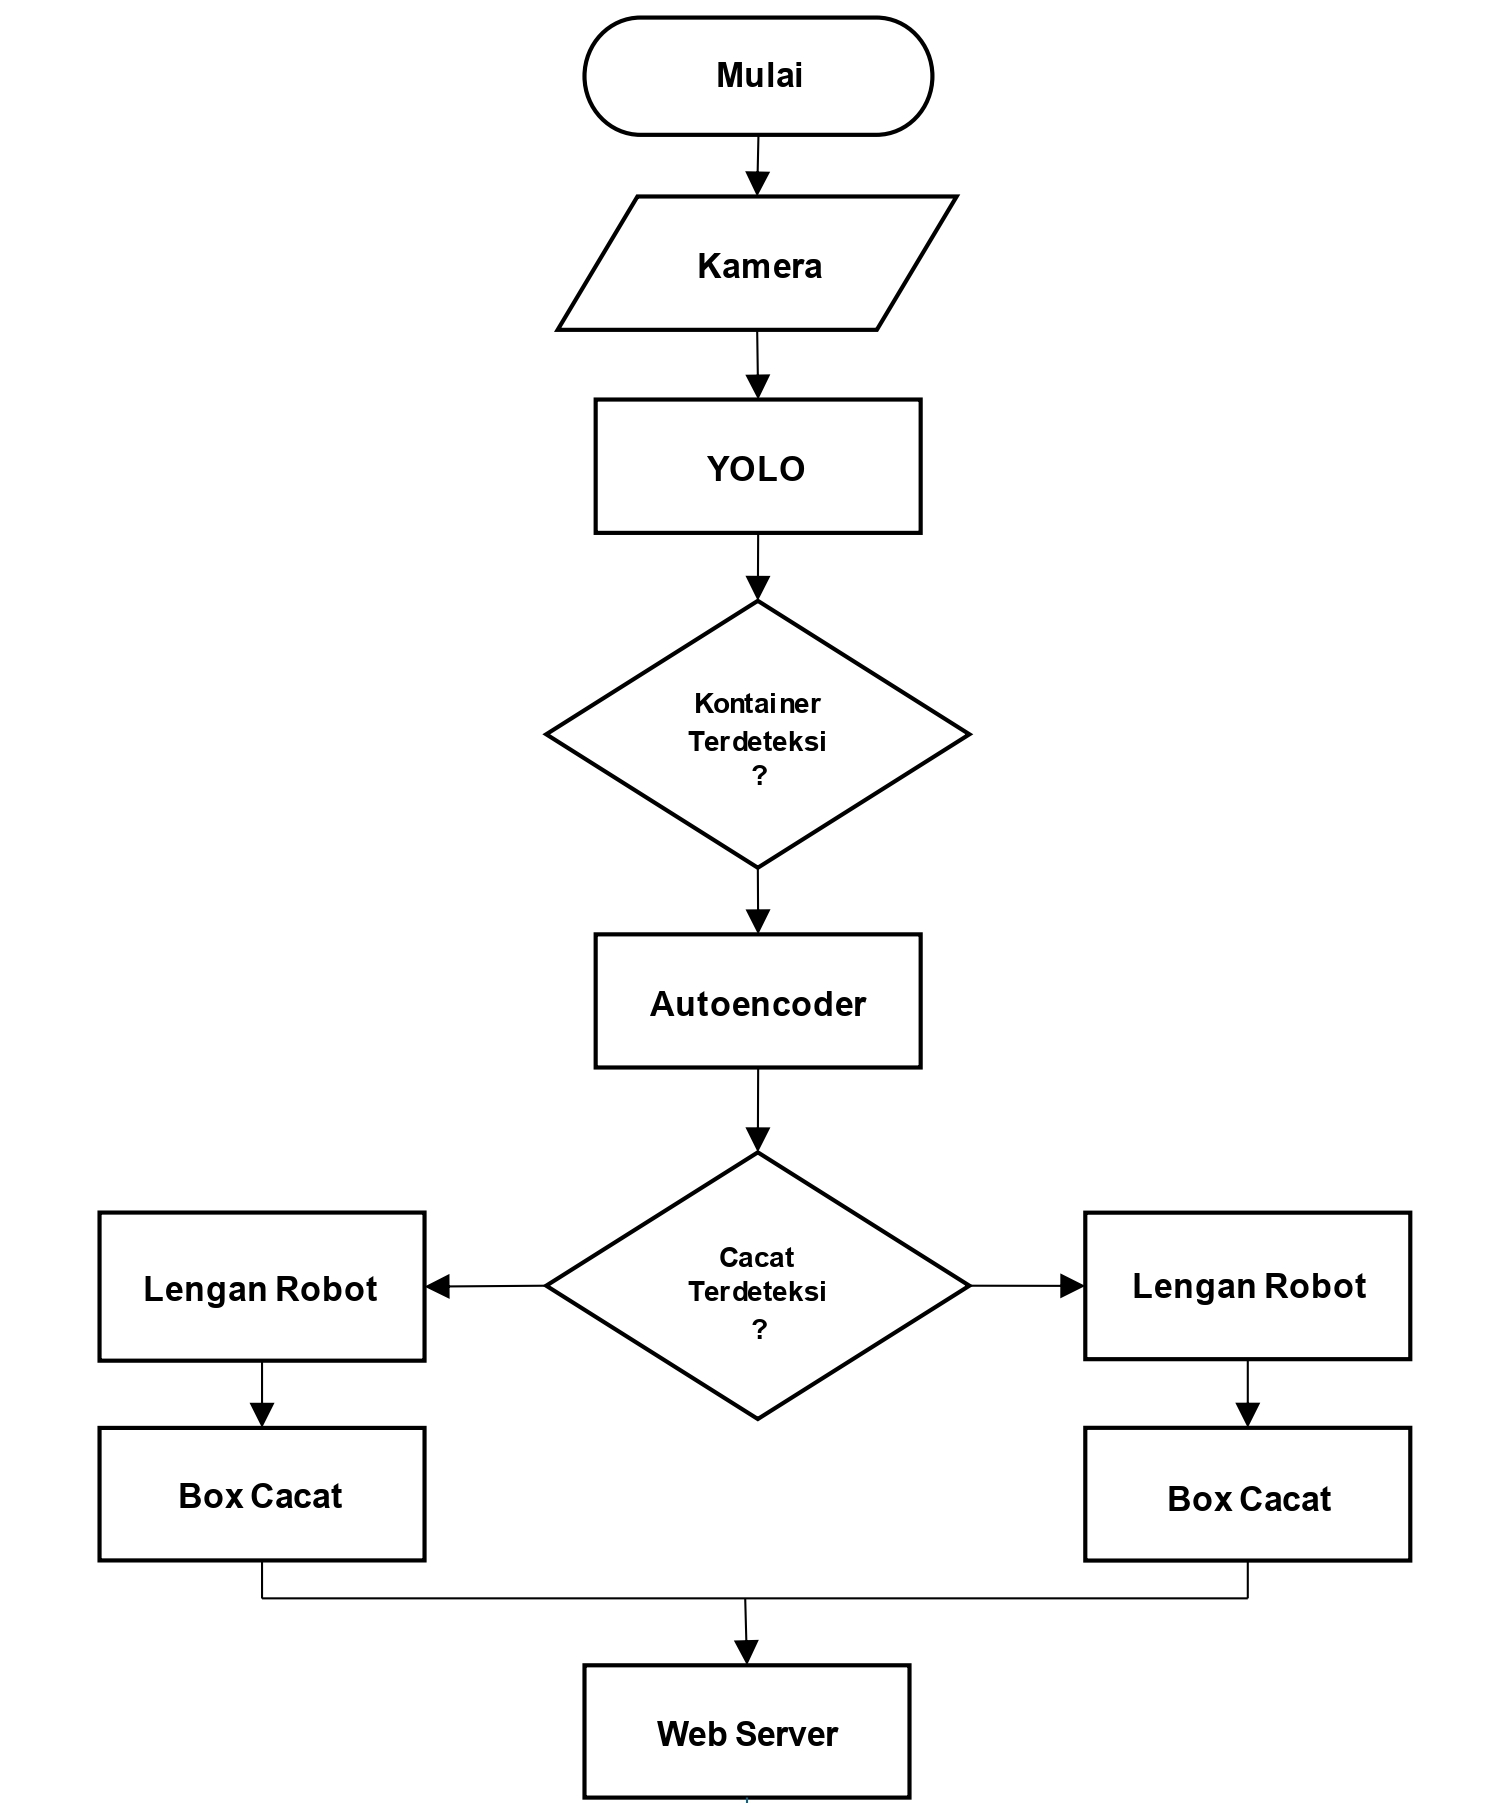
\includegraphics[]{gambar/flowchart.jpg}
  \caption{Bagan alir penelitian}
  \label{fig:bagan-alir}
\end{figure}
\vspace{-1em}

Tahapan dimulai dengan kajian mendalam terhadap teknologi robotik,
algoritma Autoencoder untuk deteksi anomali visual, serta metode
deteksi objek seperti YOLO (You Only Look Once), guna memperoleh
pemahaman komprehensif tentang konsep dasar, format dataset, dan
teknik perancangan model untuk mendeteksi cacat pada kontainer kimia.
Setelah pemahaman awal diperoleh, dilakukan perancangan sistem yang
mencakup perangkat keras (lengan robot dan sensor) serta perangkat
lunak berupa algoritma machine learning. Selanjutnya, sistem robot
dikalibrasi agar dapat bekerja secara optimal, termasuk proses tuning
hyperparameter pada model pembelajaran mesin. Jika sistem telah
berfungsi sesuai dengan yang diharapkan, maka dilanjutkan dengan
proses pengambilan data sebagai langkah awal dalam pengujian dan
validasi model.

\vspace{1em}

\subsection{Perancangan \textit{Hardware}}
Penelitian ini dimulai dengan tahap perancangan hardware. Komponen
hardware yang digunakan meliputi kamera untuk mengambil gambar
kontainer kimia, laptop sebagai pusat pemrosesan dan eksekusi
algoritma pembelajaran mesin, serta motion sensor untuk menghitung
jumlah kontainer kimia, baik yang cacat maupun yang tidak. Adapun
rancangan hardware dapat dilihat pada Gambar \ref{fig:rangkaian}.

\begin{figure}[H]
  \centering
  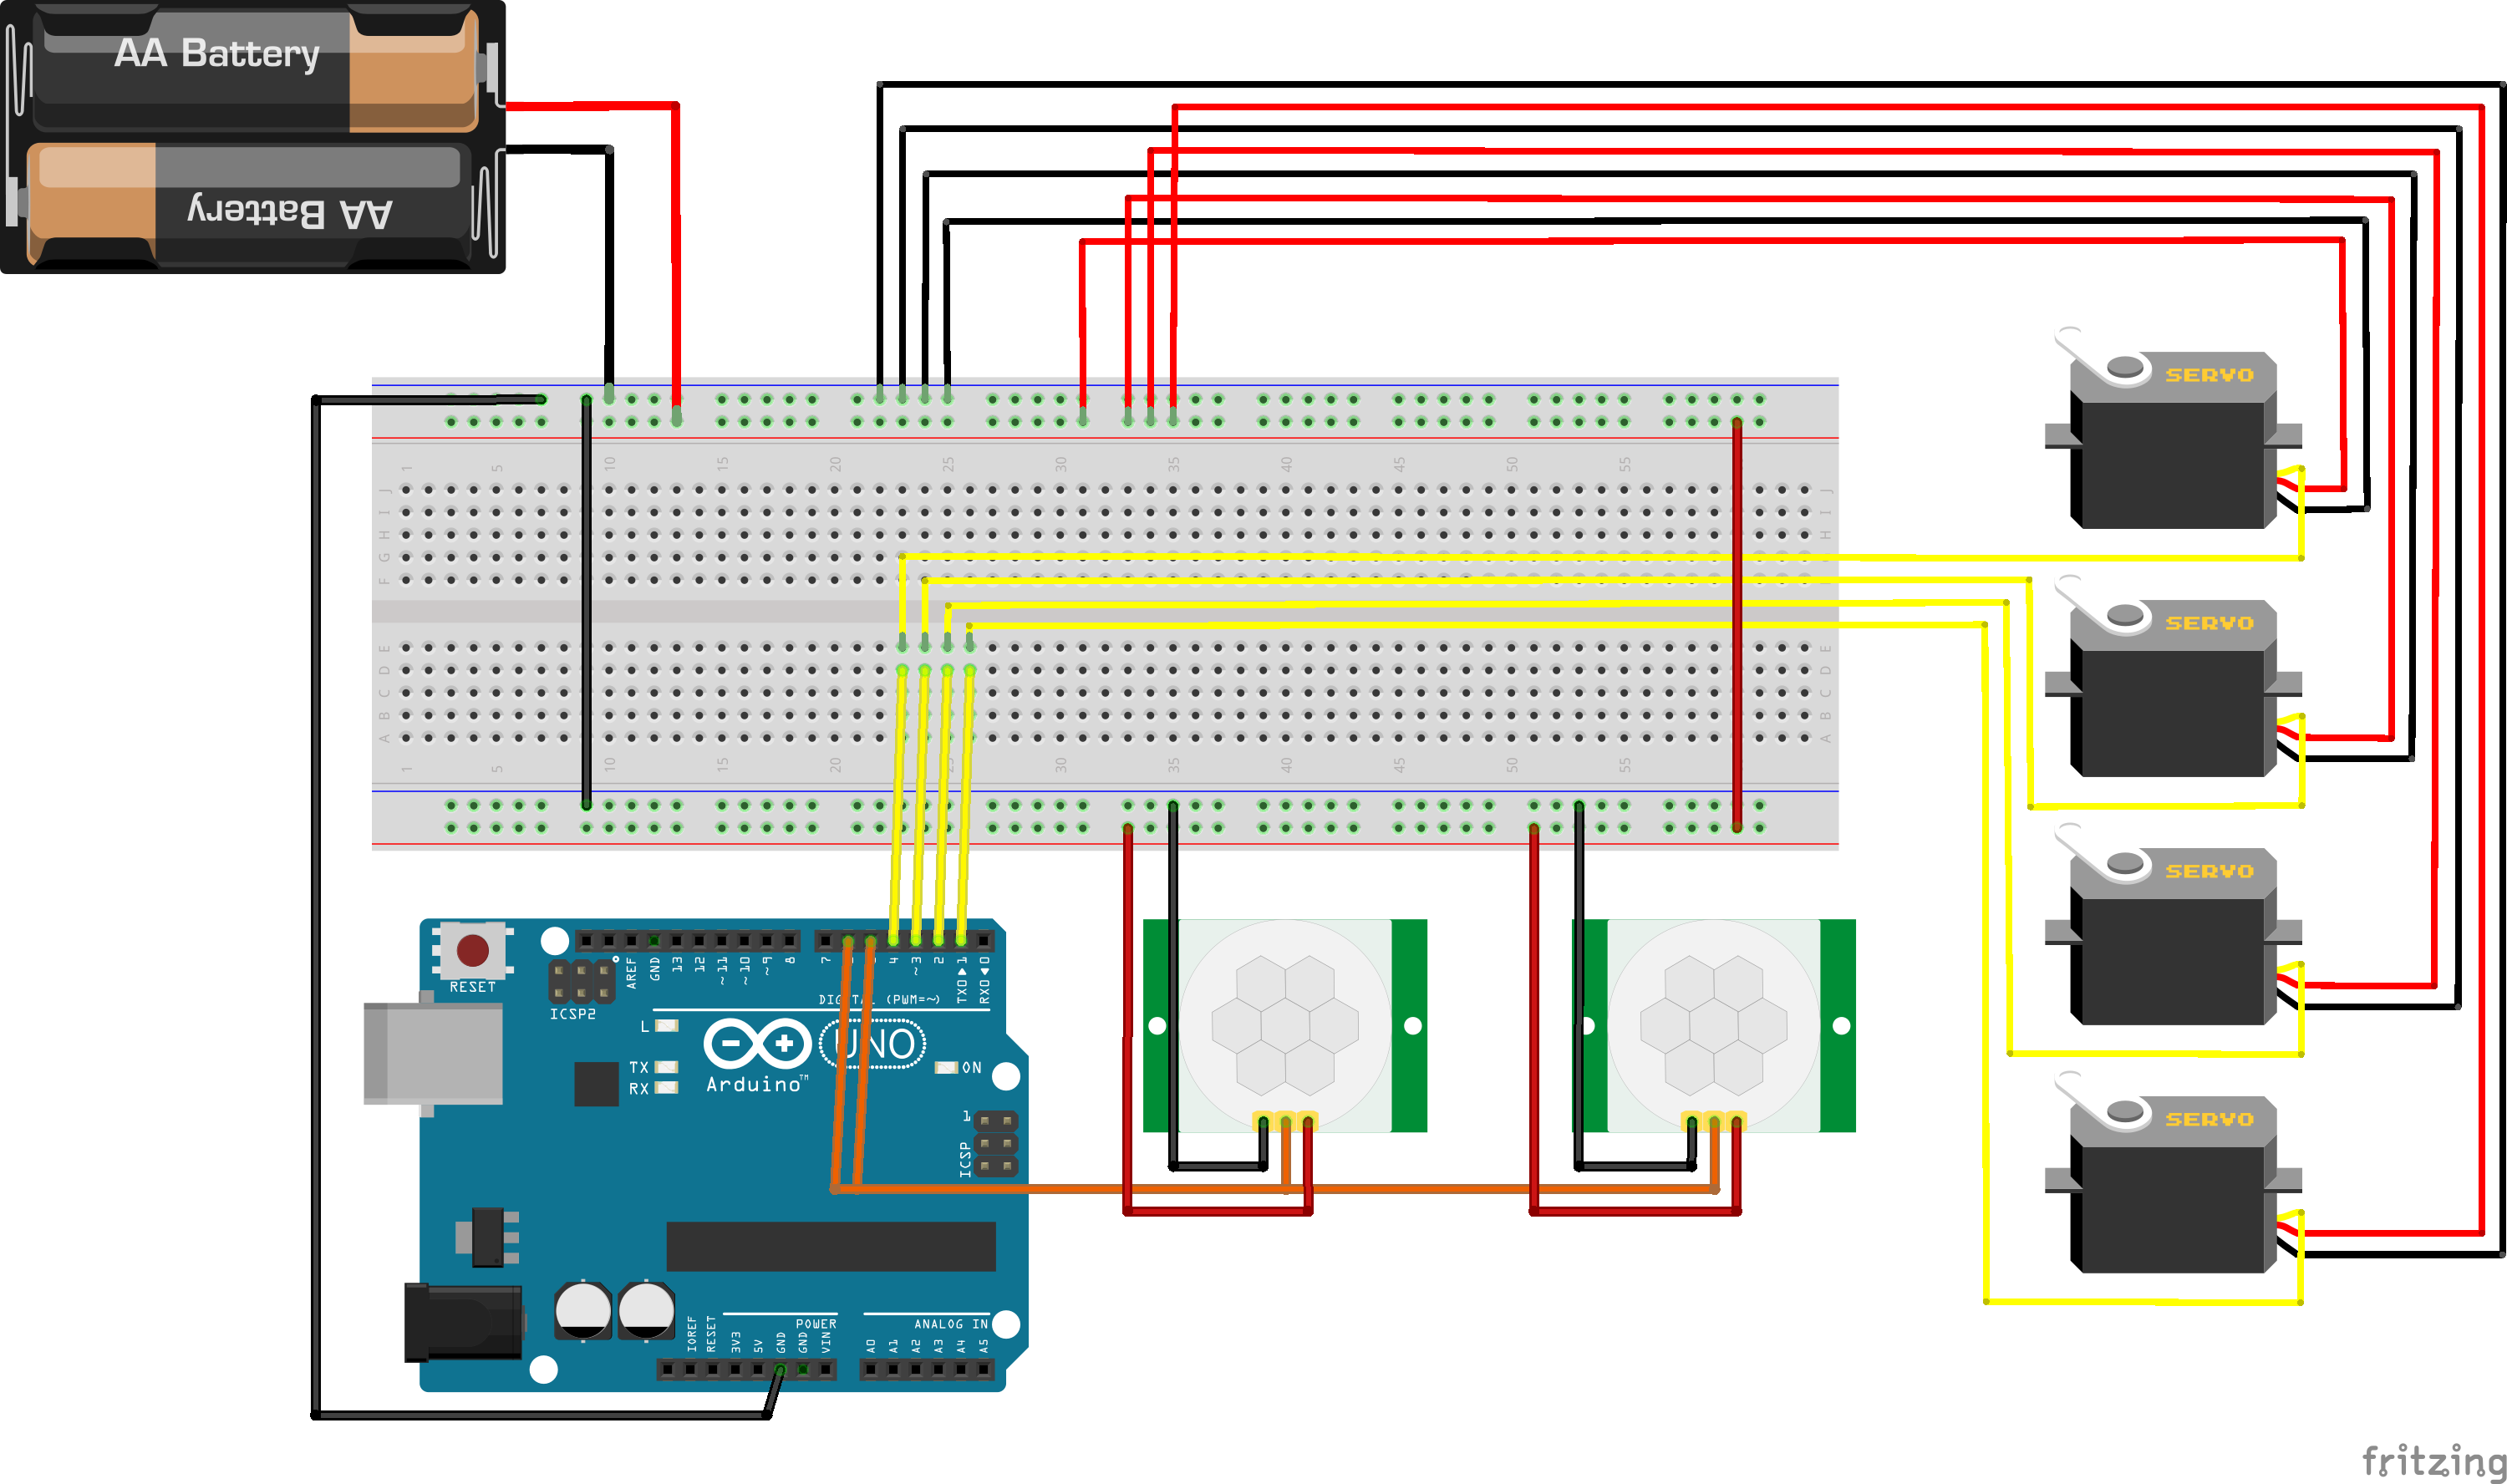
\includegraphics[width=\textwidth]{gambar/rangkaian.png}
  \caption{Bagan alir penelitian}
  \label{fig:rangkaian}
\end{figure}
\vspace{-1em}

Sistem diawali saat kamera menangkap gambar kontainer kimia yang
diletakkan di area pengambilan gambar. Gambar ini diproses oleh model
deteksi objek (YOLO) untuk mengenali keberadaan kontainer sebelum
tahap deteksi cacat. Selanjutnya, gambar yang telah dikenali dikirim
ke model deteksi kecacatan berbasis Convolutional Autoencoder untuk
menentukan apakah kontainer mengalami cacat atau tidak. Berdasarkan
hasil analisis tersebut, sinyal dikirimkan ke mikrokontroler Arduino
untuk menggerakkan servo sebagai respon terhadap kondisi kontainer.
Lengan robot kemudian mengambil kontainer kimia dan memindahkannya ke
wadah yang sesuai, tergantung pada hasil deteksi—apakah kontainer
tersebut cacat atau tidak. Untuk memantau dan menghitung jumlah
kontainer yang telah dipindahkan, dua motion sensor dipasang pada
masing-masing wadah (cacat dan noncacat). Data dari sensor ini
dikirim ke web server, yang menyediakan API untuk dikonsumsi agar
data jumlah kontainer dapat ditampilkan ke klien secara real-time.
Secara keseluruhan, keterkaitan antar komponen perangkat keras dalam
sistem ini dapat dilihat pada Gambar \ref{fig:hardware}.

\begin{figure}[H]
  \centering
  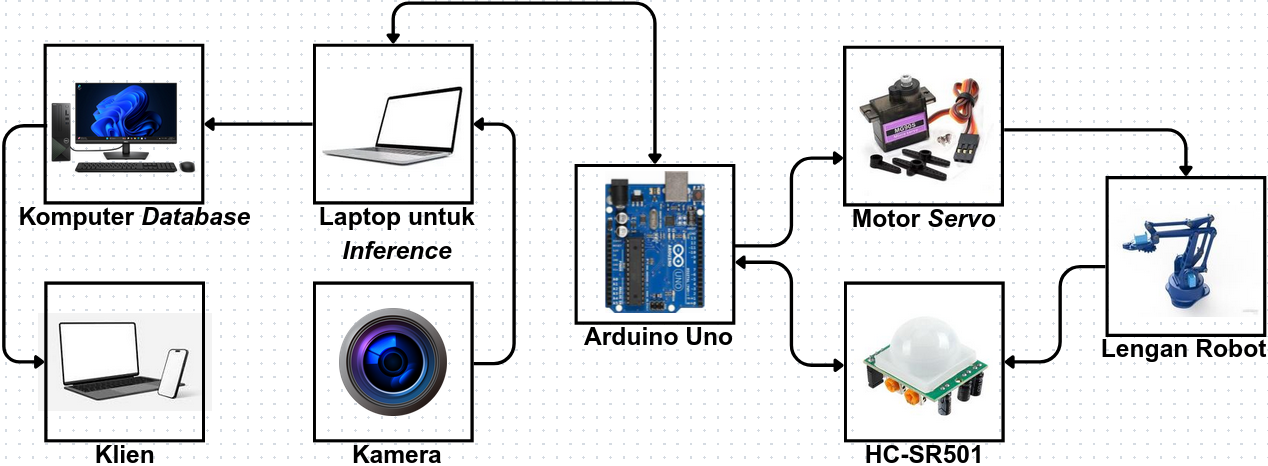
\includegraphics[width=\textwidth]{gambar/rancang.png}
  \caption{Rancang sistem \textit{hardware}}
  \label{fig:hardware}
\end{figure}
\vspace{-1em}

\vspace{1em}

\subsection{Perancangan \textit{Software}}
Perangkat lunak dalam penelitian ini mencakup perancangan beberapa
algoritma inti. Pertama, dirancang model deteksi objek berbasis YOLO
untuk mengenali kontainer kimia pada citra yang diambil oleh kamera.
Kedua, digunakan Convolutional Autoencoder sebagai model untuk
mendeteksi cacat atau anomali visual pada kontainer. Selain itu,
dirancang pula algoritma kontrol untuk mengatur pergerakan lengan
robot dalam mengambil dan memindahkan kontainer berdasarkan hasil
klasifikasi. Sistem ini juga terintegrasi dengan modul IoT untuk
menampilkan data kontainer cacat dan non-cacat pada klien secara real-time. \par

Tahap perancangan model deteksi objek dimulai dengan pengumpulan
dataset berupa gambar kontainer kimia dari berbagai kondisi dan sudut
pandang menggunakan kamera, yang nantinya dipasang bersama lengan
robot. Setelah gambar terkumpul, dilakukan proses anotasi dengan
memberikan label dan bounding box pada setiap kontainer sesuai dengan
format yang dibutuhkan oleh algoritma YOLO. Dataset yang telah
dianotasi kemudian digunakan untuk melatih model deteksi objek.
Tujuannya agar model mampu mendeteksi kontainer kimia secara akurat
dan cepat dalam berbagai situasi, misalnya ketika kontainer berada
dalam posisi miring. Setelah proses pelatihan selesai, model
dievaluasi menggunakan data uji yang belum pernah dilihat sebelumnya.
Evaluasi dilakukan menggunakan beberapa metrik seperti precision,
recall, dan mean Average Precision (mAP), guna memastikan bahwa model
memiliki kemampuan generalisasi yang baik dan layak diterapkan di
sistem robotik secara real-time. Pipeline perancangan model deteksi
objek dapat dilihat pada Gambar \ref{fig:pipeline-yolo}.

\begin{figure}[H]
  \centering
  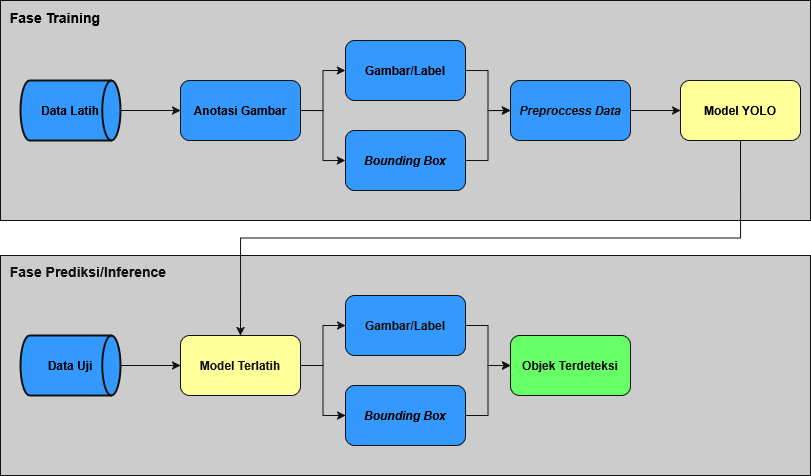
\includegraphics[width=\textwidth]{gambar/pipeline_yolo.png}
  \caption{Diagram \textit{pipeline} pelatihan model YOLO}
  \label{fig:pipeline-yolo}
\end{figure}
\vspace{-1em}

Berikutnya adalah tahap pembangunan model deteksi cacat menggunakan
algoritma Convolutional Autoencoder. Tahap ini menggunakan dataset
yang sama seperti yang digunakan pada pelatihan model YOLO, namun
tanpa menggunakan anotasi bounding box karena sifat unsupervised dari
autoencoder. Data diproses melalui tahap preprocessing seperti
resizing, normalisasi, dan augmentasi (rotasi, flipping, pencahayaan)
untuk meningkatkan variasi. Model dirancang dengan dua komponen
utama: encoder untuk mengekstraksi fitur penting dan menghasilkan
representasi berdimensi rendah (latent space), serta decoder untuk
merekonstruksi gambar dari representasi tersebut. Setelah arsitektur
selesai dan data siap, model dilatih untuk meminimalkan perbedaan
antara gambar asli dan hasil rekonstruksi, sehingga mampu mengenali
citra normal secara akurat. Evaluasi dilakukan dengan menghitung
reconstruction error, yang digunakan untuk membedakan antara gambar
normal dan cacat. Ambang batas deteksi ditentukan melalui analisis
distribusi error pada data validasi. Pipeline perancangan model
deteksi cacat dapat dilihat pada Gambar \ref{fig:pipeline-autoencoder}.

\begin{figure}[H]
  \centering
  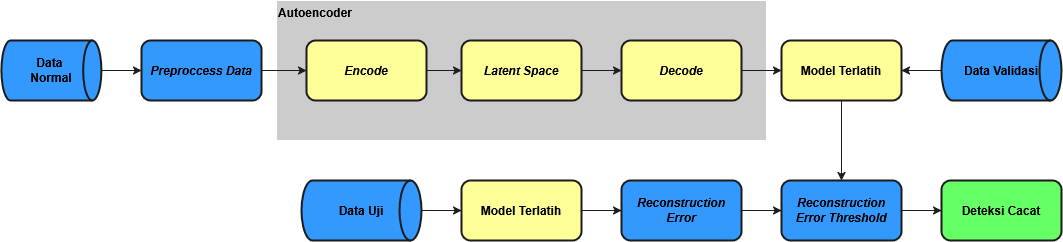
\includegraphics[width=\textwidth]{gambar/pipeline_autoencoder.png}
  \caption{Diagram \textit{pipeline} pelatihan model deteksi cacat}
  \label{fig:pipeline-autoencoder}
\end{figure}
\vspace{-1em}

\vspace{1em}

\subsection{Bagan Alir Sistem Kerja Alat}
Bagan alir sistem kerja alat terdiri dari 2 bagian yakni sistem slot
parkir dan sistem gerbang parkir. Perancangan bagan alir sistem kerja
alat secara keseluruhan ditunjukkan pada Gambar \ref{fig:bagan-alir-kerja}.

\begin{figure}[H]
  \centering
  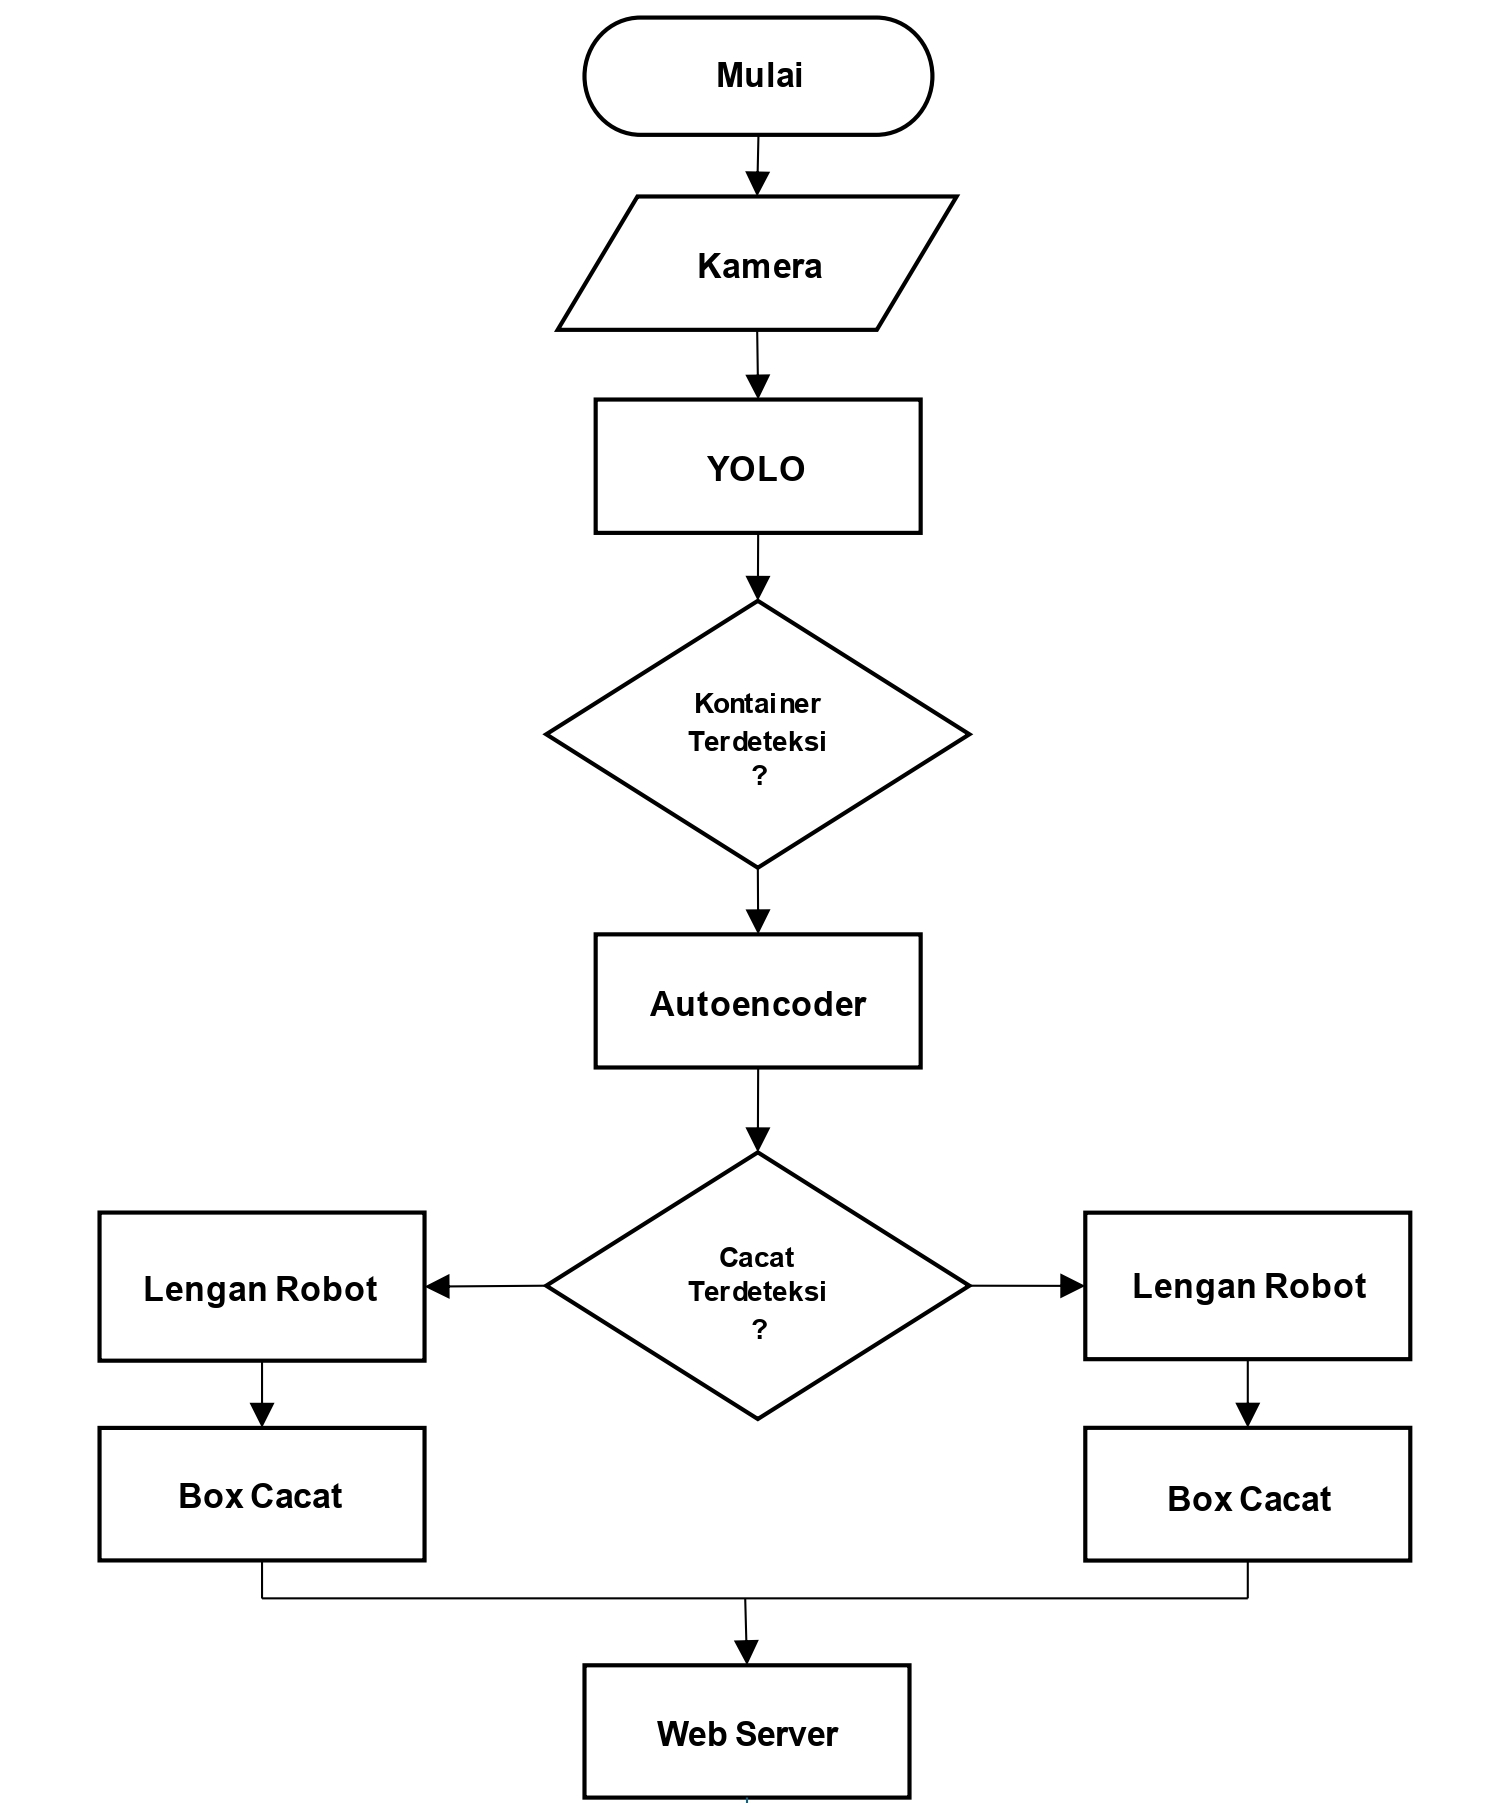
\includegraphics[]{gambar/flowchart.jpg}
  \caption{Bagan alir sistem kerja alat}
  \label{fig:bagan-alir-kerja}
\end{figure}
\vspace{-1em}
